\section{Results}

\subsection{Real GDP Forecast}
    
    The end result of our model - a multi-step forecast of GDP - is tabulated 
    out six quarters in Table \ref{tab:forecast}.  A plot is shown in Fig. 
    \ref{fig:rgdp-forecast}.
    
    The results are unsurprising but not terribly inspired. The model 
    predictions are almost indistinguishable from a linear extrapolation over the
    last four quarters.  Also disappointing are the confidence thresholds, which
    grow substantially with each step in the forecast.

    \begin{table}[!h]
        \centering
        \begin{tabular}{c c c} 
            \bf{Quarter} & \bf{Forecast} & \bf{95\% Conf. Interval} \\ \hline
            2016-Q1 & 16.563 & 16.339 - 16.789 \\
            2016-Q2 & 16.687 & 16.330 - 17.051 \\
            2016-Q3 & 16.805 & 16.315 - 17.310 \\
            2016-Q4 & 16.919 & 16.309 - 17.552 \\
            2017-Q1 & 17.028 & 16.296 - 17.794 \\
            2017-Q2 & 17.136 & 16.293 - 18.023 \\
        \end{tabular}
        \caption{Forecasted U.S. GDP from 2016Q1 to 2017Q2}
        \label{tab:forecast}
    \end{table}
    
    \begin{figure}
        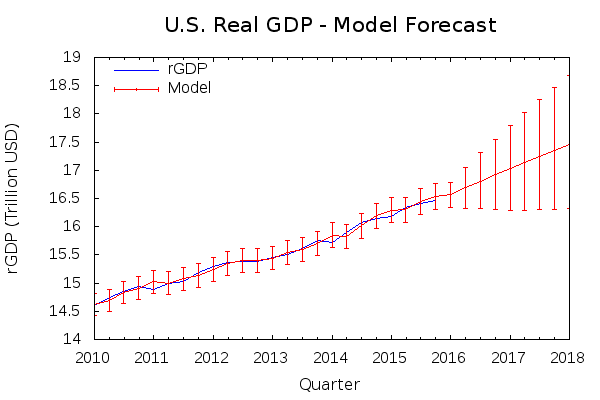
\includegraphics[width=\textwidth]{../img/model1-rgdp-forecast.png}
        \caption{Forecasted U.S. GDP from 2016-2018}
        \label{fig:rgdp-forecast}
    \end{figure}

\subsection{Analyzing Outliers}

    One interesting feature of the model is the historical distribution of GDP residuals
    (prediction errors), shown in Fig. \ref{fig:residuals}.  Note that outliers 
    occur mostly around recessionary periods:
    \begin{itemize}
        \item 1970-Q4, 1971-Q1: just after recessionary period (Dec 1969 - Nov 1970)
        \item 1980-Q2, 1980-Q4: during recessionary period (Jan - Jul 1980)
        \item 2008-Q4: during sub-prime mortgage crisis
    \end{itemize}
    
    This is unsurprising, given that recessions are hard to predict even with
    the most sophisticated models.
    
    \begin{figure}[!h]
        \begin{center}
        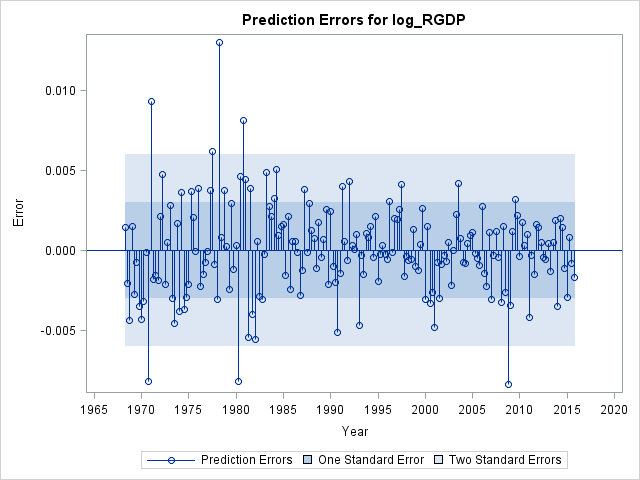
\includegraphics[width=0.8\textwidth]{../img/model1-residuals.png}
        \end{center}
        \caption{Model GDP residuals from 1967-2015}
        \label{fig:residuals}
    \end{figure}
    

\section{Conclusions}
   
    We constructed a basic VAR(4) model of U.S. real GDP that performed well with
    historical data but provided only limited predictive insights.  It forecasts
    linear economic growth for at least the next four quarters, through Q1 2018.
    However, the large uncertainty bounds make forecasting of more than one
    or two quarters ahead meaningless.  The model also notably
    fails to predict many historical economic recessions.
    
    We posit that a much more sophisticated model is necessary to anticipate
    real movements in GDP before they happen.  This includes a better framework -
    perhaps a Vector Autoregressive Moving Average model - as well as more 
    carefully tuned choice of variables.